\documentclass{article}
\usepackage{cmap}
\usepackage[utf8]{inputenc}
\usepackage[english,ukrainian]{babel}
\usepackage{graphicx}
\usepackage{geometry}
\usepackage{listings}
\usepackage{float}
\usepackage{amsmath}
\usepackage{subfig}
\usepackage{xcolor}
\geometry{
	a4paper,
	left=20mm,
	right=20mm,
	top=15mm,
	bottom=15mm,
}
\lstset{
	tabsize=4,
	keepspaces,
	showstringspaces=false,
	escapeinside={(*@}{@*)},
}
\graphicspath{ {./pictures} }
\setlength{\parindent}{4em}

\newcommand\subject{Архітектура комп'ютера}
\newcommand\lecturer{доцент кафедри ПЗ\\Крук О.Г.}
\newcommand\teacher{доцент кафедри ПЗ\\Крук О.Г.}
\newcommand\mygroup{ПЗ-22}
\newcommand\lab{6}
\newcommand\theme{Опрацювання рядка символів засобами асемблера мікропроцесорів х86. Робота з файлами}
\newcommand\purpose{Освоїти команди асемблера для роботи з рядками символів; опанувати функції Win32 для роботи з файлами; розвинути навики складання програми для опрацювання рядка символів та програми для створення, записування і читання текстового файла; відтранслювати і виконати в режимі відлагодження програми, складені відповідно до свого індивідуального завдання}

\begin{document}
\begin{normalsize}
	\begin{titlepage}
		\thispagestyle{empty}
		\begin{center}
			\textbf{МІНІСТЕРСТВО ОСВІТИ І НАУКИ УКРАЇНИ\\
				НАЦІОНАЛЬНИЙ УНІВЕРСИТЕТ "ЛЬВІВСЬКА ПОЛІТЕХНІКА"}
		\end{center}
		\begin{flushright}
			\textbf{ІКНІ}\\
			Кафедра \textbf{ПЗ}
		\end{flushright}
		\vspace{200pt}
		\begin{center}
			\textbf{ЗВІТ}\\
			\vspace{10pt}
			до лабораторної роботи № \lab\\
			\textbf{на тему}: “\textit{\theme}”\\
			\textbf{з дисципліни}: “\subject”
		\end{center}
		\vspace{112pt}
		\begin{flushright}
			
			\textbf{Лектор}:\\
			\lecturer\\
			\vspace{28pt}
			\textbf{Виконав}:\\
			
			студент групи \mygroup\\
			Коваленко Д.М.\\
			\vspace{28pt}
			\textbf{Прийняв}:\\
			
			\teacher\\
			
			\vspace{28pt}
			«\rule{1cm}{0.15mm}» \rule{1.5cm}{0.15mm} 2022 р.\\
			$\sum$ = \rule{1cm}{0.15mm}……………\\
			
		\end{flushright}
		\vspace{\fill}
		\begin{center}
			\textbf{Львів — 2022}
		\end{center}
	\end{titlepage}
		
	\begin{description}
		\item[Тема.] \theme.
		\item[Мета.] \purpose.
	\end{description}

	\section*{Індивідуальне завдання}
	\begin{figure}[H]
		\centering
		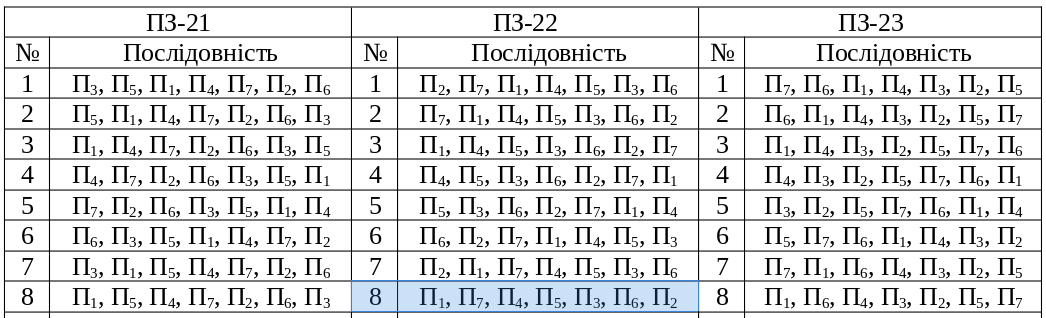
\includegraphics[scale=0.45]{v}
	\end{figure}
	
	\section*{Хід роботи}
	\subsection*{Код програми}
	\begin{lstlisting}[language={[x86masm]Assembler}]
.686 
.model flat,stdcall 
.stack 

.DATA

text2       BYTE 105 DUP (?)
text3       BYTE 75 DUP (?)

field1      BYTE 22 DUP (?)
field2      BYTE 22 DUP (?)
field3      BYTE 22 DUP (?)
field4      BYTE 22 DUP (?)
field5      BYTE 22 DUP (?)
field6      BYTE 22 DUP (?)
field7      BYTE 22 DUP (?)

field1Len   DWORD ?
field2Len   DWORD ?
field3Len   DWORD ?
field4Len   DWORD ?
field5Len   DWORD ?
field6Len   DWORD ?
field7Len   DWORD ?

spacesTotal DWORD 0
wordStart   DWORD 0

.CODE
spacesLen PROC start:DWORD
mov EDI, OFFSET text
add EDI, start
mov ESI, EDI
mov AL, ' '
mov ECX, 75
repe scasb      
dec EDI
sub EDI, ESI
mov EAX, EDI
mov EBX, EAX
add EBX, start
ret             
spacesLen ENDP

fieldLen PROC start:DWORD  
mov EAX, start
mov wordStart, EAX
mov EDI, OFFSET text
add EDI, start
mov ESI, EDI
mov AL, ' '
mov ECX, 75
repne scasb     
dec EDI
sub EDI, ESI       
mov EAX, EDI
mov EBX, EAX
add EBX, start
ret      
ret
fieldLen ENDP

main PROC
invoke fieldLen, 0
mov field1Len, EAX   

mov ECX, field1len  
mov ESI, OFFSET text
mov EDI, OFFSET field1
rep movsb

invoke spacesLen, EBX
add spacesTotal, EAX   

invoke fieldLen, EBX   
mov field2Len, EAX

mov ECX, field2len
mov ESI, OFFSET text
add ESI, wordStart
mov EDI, OFFSET field2
rep movsb

invoke spacesLen, EBX
add spacesTotal, EAX

invoke fieldLen, EBX  
mov field3Len, EAX

mov ECX, field3len
mov ESI, OFFSET text
add ESI, wordStart
mov EDI, OFFSET field3
rep movsb

invoke spacesLen, EBX
add spacesTotal, EAX

invoke fieldLen, EBX  
mov field4Len, EAX

mov ECX, field4len
mov ESI, OFFSET text
add ESI, wordStart
mov EDI, OFFSET field4
rep movsb

invoke spacesLen, EBX
add spacesTotal, EAX

invoke fieldLen, EBX  
mov field5Len, EAX

mov ECX, field5len
mov ESI, OFFSET text
add ESI, wordStart
mov EDI, OFFSET field5
rep movsb

invoke spacesLen, EBX
add spacesTotal, EAX

invoke fieldLen, EBX  
mov field6Len, EAX

mov ECX, field6len
mov ESI, OFFSET text
add ESI, wordStart
mov EDI, OFFSET field6
rep movsb

invoke spacesLen, EBX
add spacesTotal, EAX

invoke fieldLen, EBX  
mov field7Len, EAX

mov ESI, OFFSET text
add ESI, wordStart
mov EDI, OFFSET field7
mov ECX, field7len
rep movsb

invoke spacesLen, EBX
add spacesTotal, EAX

mov AL, ' '
mov EDI, OFFSET text2

mov ECX, 1
rep stosb
mov ESI, OFFSET field1
mov ECX, field1len
rep movsb

mov ECX, 7
rep stosb
mov ESI, OFFSET field7
mov ECX, field7len
rep movsb

mov ECX, 4
rep stosb
mov ESI, OFFSET field4
mov ECX, field4len
rep movsb

mov ECX, 5
rep stosb
mov ESI, OFFSET field5
mov ECX, field5len
rep movsb

mov ECX, 3
rep stosb
mov ESI, OFFSET field3
mov ECX, field3len
rep movsb

mov ECX, 6
rep stosb
mov ESI, OFFSET field6
mov ECX, field6len
rep movsb

mov ECX, 2
rep stosb
mov ESI, OFFSET field2
mov ECX, field2len
rep movsb
ret
main ENDP

END main
	\end{lstlisting}


	\section*{Висновки}
	Під час виконання лабораторної роботи я освоїв команди асемблера для роботи з рядками символів; опанував функції Win32 для роботи з файлами; розвинув навики складання програми для опрацювання рядка символів та програми для створення, записування і читання текстового файла; відтранслював і виконати в режимі відлагодження програми, складені відповідно до свого індивідуального завдання.
	    
\end{normalsize}
\end{document}
